\documentclass{report}

%Document Preamble
\usepackage[utf8]{inputenc}
\usepackage[a4paper, portrait, margin=1.5in]{geometry}
\usepackage{graphicx}
\usepackage{float}
\usepackage{sectsty}
\usepackage[normalem]{ulem}
\usepackage{booktabs}
\usepackage{draftwatermark}
\SetWatermarkText{FINAL DRAFT}
\SetWatermarkScale{4}
\useunder{\uline}{\ul}{}

\graphicspath{{img/}}

\chapternumberfont{\LARGE} 
\chaptertitlefont{\Large}
\sectionfont{\large}
\subsectionfont{\normalsize}

\title{\textbf{LectureMate} \vspace{0.5cm} \hrule \vspace{0.5cm}Final Draft Project Report}
\author{\textbf{Manpreet Singh Bance | 33552762}}
\date{May 2020}

\begin{document}
\maketitle

\tableofcontents
\newpage

\thispagestyle{empty}
\listoffigures
 
\listoftables

\newpage
\section*{Acknowledgements}

I would like to express my gratitude towards my supervisor, Golnaz Badkobeh, for her continued support and guidance throughout the course of the entire project, providing assistance from preparing the project for development to project completion.\\

I would also like to thank my family for their support in my studies throughout the duration of this degree.  \\

\par Finally, I would like to thank Lahcen Ouarbya, and the Department of Computing at Goldsmiths, University of London, for the opportunity to work on this project.

\chapter{Introduction}
LectureMate is designed to be a cross-platform mobile application for use in an educational setting, namely, lectures - whereby, students and other academics can use the application to make dynamic, powerful and relevant notes which are linked to a specific timestamp or set of timestamps. The type of notes which can be made are rich text, uploaded images or camera photos, links, documents/research papers - all of which would the user would deem to be relevant to the point of the audio recording which is being made. As well as this, the user has the ability to highlight certain segments in the audio which they feel are important and they would benefit from later on when coming back to review these notes, for example, during revision.\\

As previously mentioned, the mobile app is mainly aimed at educators and academics in the educational setting but due to its capabilities could potentially be used in a range of other settings. Primary research showed that there were no existing applications on the market which offered the functionality that this mobile application aims to do. Existing applications such as Evernote are based primarily on text-based notes with the ability to add further attachments, whereas LectureMate would be audio-based allowing for notes to be made based on the timestamp in the audio recording.\\

Secondary research was able to prove that educators (the primary target market) and among students at Goldsmiths College, University of London, that there was no one consistent form of making clear, relevant notes and that the target market relied on a number of various applications to make notes which was not a practical solution. These applications incliuded the likes of Evernote, Microsoft OneNote, Google Docs, as well as traditional notes which were made with pen and paper which were later difficult to merge with existing notes on these applications.\\

From this, it was clear that the application would aim to provide a satisfactory solution to the needs of the market and honoring what is in need by the target market which was able to be identified through the research. As a result, upon deployment of the application we would be able to see whether this is fulfilled and is versatile enough to meet the needs of its users. This is evidence to show how an application and platform such as LectureMate is vital in filling a much needed gap in the market.

	\section{Motivation}
The motivation behind this mobile applcation is upon research the lack of platforms which allow users to make notes based on audio recordings. As well as this, in first-hand experience, I was able to identify that I found note-taking particularly inconsistent and upon coming back to these notes to revise I found these notes to have no context and difficult to understand. Therefore, I carried out some research to see whether any platforms existed which allowed notes to be made but with some context and found that there were none for wide use.\\

By this and by communicating with peers among different educational settings, I was able to recognise that most univerities and lecture theatres had recording equipment. I initially upon ideation, thought of pursuing this, however, later came to the conclusion that this would not be a viable option due to the issues with obtaining the permission of those individuals who may be visible in the recording, and as a result I made the final decision to proceed with the same idea however, using audio recording instead.

	\section{Scope}
LectureMate aims to combat the issues that students and academics face in the note-taking and revision aspect of their learning by providing a platform where they can make clear, dynamic and consistent notes in order to tackle the existing problems faced with making notes where the notes are made across different platforms making them different to compile and are inconsistent. Therefore, making clear, consistent and dynamic notes using LectureMate are a solution to these issues.

	\section{Objectives}
One of the first things which were looked at was how we can meet the objective to fulfill the need for the target market which was identified. LectureMate does this by providing a platform to satisfy the need for making clear notes.\\

We needed to make sure that the application met the needs that our target market fed back to us when conducting our primary and secondary ressearch. Another objective that was indicated through executing this research was that the application would have the ability to highlight specific points within the audio where upon reviewing, would be able to identify the key, relevant sections of a lecture or recording.\\

The security and integrity of the notes which are made are a priority as these notes are to be kept safe whereby unauthorised changes should not be made to the notes as well as their security being ensured as to them not becoming deleted or corrupted. Therefore, considering this, the app aims to be a safe and reliable platform for its users so that they do not need to worry about the integrity of their notes. The application will do this by saving the note as a file in a folder creating regular backups each day or manually.\\

As the files will be stored locally on the device, the user is responsible for any data which might be subject to any tampering or corruption to the files when being manipulated through any third party application such as a file explorer. Using the application to make any changes to any notes will be a tested and safe way for users to alter notes.

\chapter{Technical Specification}
	\section{Background Research}
	Here, I will focus and discuss the research I carried out prior to commencement of the design of the application. I will begin technical research looking at the potential for technologies I may use to develop the mobile application and briefly address the reasons behind this.

		\subsection{Existing Systems}
In the research stage, I wanted to explore the market for existing applications which perform or complete similar or exactly the functions that I was aiming for in this application. I decided to look at features I would be able to implement from others or simply known, working models which wre proven to be good applications and have relevant, useful features I could also implement. However, I wanted to be inspired by these and not just implement the feature in the same way as the app I would be borrowing from.
			\subsubsection{Soundcloud}\cite{Soundcloud}
While doing research, I thought of existing systems which I can obtain certain features from which I might be able to incorporate into the mobile application. Soundcloud came to mind whereby in their interface, they have the ability to have their users to add comments at certain time points in the audio which had been uploaded. I thought this same model would be able to be applied to this application as notes can be added at a specific point in the audio recording.
			\subsubsection{Evernote}
Again, whilst looking at exisitng applications, if not one of the biggest, is Evernote who provide a cross-platform note taking solution. I therefore studied this application well and listed features I also look to implement into this application - these included: the ability to upload images, audio attachments and links. These features would all be very useful in a note taking setting, especially in a lecture setting.

	\section{Overview}
The technical architecture of the mobile application is as simple as the layering mode. The logic of a layered architecture allows the separation of the Front-End, Middleware and Back-End, however still allowing for cohesion between these, which will be detailed further.\\

The uppermost layer will be the presentation layer - which will be the appearance and interaction side of the application, the middle layer - which will be responsible for the (business) logic behind the application containing the code behind the actions interacted with in the presentation layer, and the data access layer - which will be the back end code which enables the user to access and make changes to the notes, although stored locally, they will still carry out CRUD functionality similar to that used in databases.

	\section{Application Frameworks}
A framework is an abstraction where software is written to provide generic function to achieve a task or tasks. This mobile application has made use of some frameworks to contribute to the functioning of it - mainly being in the Front-End or 'Presentation Layer'.

	\section{Full Stack Development}
As previously mentioned, the web application was designed and structured in a way conforming to the stack structure: Front-End, Middleware, and Back-End. This section will further discuss the specification of technologies in each tier of the stack and the reasons behind their uses: 

		\subsection{Flutter}
The entirety of the mobile application will be using the existing Flutter framework which is an open-source UI software development kit created by Google - used to develop applications across mobile, web and desktop applications. I will detail the framework architecture and the way each of these are used in the development of the mobile application: 

		\subsubsection{Dart platform}
Flutter apps are written in the Dart language and make use of many of the language's more advanced features. The Dart language package allows during development for implementing features into the application which help shape the appearance and layout as it appears to be.\\

During the development stage, the Dart package also allows for dynamic and a live coding experience which involves hot reloading whereby any changes in code can be updated and made live without having the whole application have to be restarted for the new changes to take effect which was a welcome and proven helpful feature to the process.

		\subsubsection{Flutter engine}
The flutter engine provides low-level rendering support interfacing with iOS and Android platforms which hosts the Fluttter applications and manages the way they look and behave controlling and making use of its core libraries which include animation and graphics, file and network I/O, accessibility, plugin and runtime and compilation toolchain. However, these were things which during the development process were something which were not deeply explored and only utilised for basic functionality.\\

Using the Flutter framework allowed for a more reactive, modern framework for creating a modern and engaging mobile application which would also function well.

		\subsubsection{Foundation library}
The foundation library written in Dart allowed for the use and implementation of basic classses and functions in the mobile application enabling access to APIs to communcate with the engine and construct the application.

		\subsubsection{Widgets}
Flutter widgets are built into the package and work as the different components which make up together to build the application, such as buttons and text. These are included as standard and are used in the application for some of the components.\\

Design-specific widgets such as Material design using Google's design language as well as Cupertino which use Apple's Human Interface Guidelines iOS design, both make use of these respective design langauges to display the application best in their respective, native environments to give them a more uniform look despite being on different platforms.
	
		\subsubsection{Google Firebase}
At a later stage in the implementation stage, it was concluded that issues would arise with the storage and retrieval of data, namely media such as images, videos and audio as it would be difficult to reference in using the application and it made sense to make use of a database to solve this. Due to the nature and cohesiveness due to being both Google developed systems, it would make sense to use Google Firebase as the database management.\\

This would allow for the storage of raw data such as strings and numerical characters; Firebase also has a solution for the storage of media items as this utilises Firebase storage which gives each record a unique identifier which can be associated to the respective note and would could be stored successfully.

\chapter{Project Management}

	\section{Labour/Resource Management}
Prior to commencement of the project, I planned to allocate resources in the form of time, being the number of hours spent, on each stage of the project with ideation to conception, research, development and testing stages to ensure that this was all done in good timing and enough resources were spent on each stage so that it would be produced to a high standard. Following the allocation of resoruces available throughout the project, I created a timeline with set provisional dates whereby these tasks should be completed, referred to as milestones.

Taking this approach to the allocation of labour and resources means I can plan when certain tasks should be done and if these are not met, I can allocate further resources to make the project less susceptible to interruptions, which may include:

\begin{enumerate}
\item \textbf{Overlap of tasks:}\\
The tasks were divided in smaller segments to ensure better productivity and efficiency in completing each tasks and to make sure that each task was completed correctly prior to moving onto the next task. This guaranteed that there was less of a feeling of a being stuck on a particular task for a prolonged amount of time and a wider variety to provide a faster workrate of tasks being completed. Due to the nature of the developmemt process being in Flutter, the bulk of the project was the middleware and backend controlling the way functions and features were supposed to behave and whether these were being suitably met. The tasks were divided in such a way that there was no dependency of completion of a task to complete the next as such until it came to testing to see whether these worked together cohesively.
\item \textbf{Time keeping and meeting deadlines:}\\
The time keeping and milestone aspect of the planning process was very important so that each of these were being met on time and no stage of the development process was falling behind so much so that it would not be complete and the application as a whole would suffer. To combat this, I created a blog so that I was keeping track of the developments made in the project each week to track whether this progress was good and steady and would meet the milestones at the correct times. Planning these milestones enables for a greater control of the project and the way it is progressing.
\end{enumerate}

	\section{Methodology}
		\subsection{Agile Development Method}
The Agile Project Management Methodology was utilised where, by definition, an iterative process made use of at each stage of development in all areas of the development stack requiring constant effective communication. Using the Agile method meant that the project was dealt with the most efficient way possible with larger tasks being broken down and divided as to the larger and smaller tasks taking varying time to complete and complete these tasks effectively.

		\subsection{Kanban}
The Kanban method is also used in order to keep track of the items which need to be completed and which are still yet to be completed as well as a section to review code and carry out ah-hoc testing as well as component testing to see whether each component is working as expected. This also provides a more broader look at the tasks to come and time to prepare for these, seeing whether any previous tasks are dependant or feed into the following task. The Kanban method is visualised using Trello.

	\section{Version Control}
		\subsection{Git}
The project makes strong use of Git and its features for version control purposes, with the ability to see and track any changes to files and have a history of the previous changes made and to apply any future fixes giving more of a sense of control and responsibilty for each task to be completed correctly as well as the a timestamp of when this has been completed to identify whether it has been done in good time according to the milestones and personal proposed dates.

\chapter{Analysis}
	\section{System Requirements}
	System requirements outlines the criteria needed to complete the application to a standard meeting the MVP and beyond. This is looked at in two separate sections, functional and non-functional requirements. These requirements are set here so as to build and define clear terms to avoid any misunderstanding in any of the stages of implementation which in turn allow me to predict the challenges I might face and be ready to spend more time and allocate resources here whereby I can plan time spent on each stage to clearly visualise a viable and realistic application to produce in the timeframe and to what standard I can produce tbis to.
		\subsection{Functional Requirements}
		Essentially minimum requirements the application is expected to handle and accommodate:
		\begin{table}[H]
			\begin{tabular}{|l|l|l|}
			\hline
			ID   & Description                                                                                                                                                             & \begin{tabular}[c]{@{}l@{}}Vital/Optional \\ 						Requirement\end{tabular} \\ \hline
			FR01 & Mobile application to run at least on all Android devices                                                                                                               & Vital                                                                 			\\ \hline
			FR02 & \begin{tabular}[c]{@{}l@{}}Mobile application requires constant, reliable access to internet \\ connection to user's device\end{tabular}                                & Vital                                                                 			\\ \hline
			FR03 & \begin{tabular}[c]{@{}l@{}}Mobile application user input data to be stored securely on \\ Google Firebase\end{tabular}                                                  & Vital                                                                 			\\ \hline
			FR04 & \begin{tabular}[c]{@{}l@{}}Mobile application to back up audio recordings to be stored \\ locally on device in the event of unreliable internet connection\end{tabular} 			& Optional                                                              \\ \hline
			FR05 & \begin{tabular}[c]{@{}l@{}}Mobile application should allow the user to make notes and be \\ able to retrieve and view these\end{tabular}                                & Vital                                                                 			\\ \hline
			FR06 & \begin{tabular}[c]{@{}l@{}}Mobile application should enable the user to carry out CRUD \\ functionality through the database\end{tabular}                               & Vital                                                                 			\\ \hline
			\end{tabular}
			\caption{Functional Requirements}
			\label{Functional Requirements}
		\end{table}

		\subsection{Non-functional Requirements}
		\begin{table}[H]
			\begin{tabular}{|l|l|l|}
			\hline
			ID   & Description                                                                                                                                                             & \begin{tabular}[c]{@{}l@{}}Vital/Optional \\ 						Requirement\end{tabular} \\ \hline
			NFR01 & Mobile application should run on Android or iOS mobile device & Optional                                                                 			\\ \hline
			NFR02 & \begin{tabular}[c]{@{}l@{}}Mobile application should be usable easily for any user to achieve \\the purpose of the application\end{tabular}                                & 					Vital                                                                 			\\ \hline
			NFR03 & \begin{tabular}[c]{@{}l@{}}Mobile application should store the data with integrity without the \\ability to maliciously alter data\end{tabular}                                                  			& Vital                                                                 			\\ \hline
			NFR04 & \begin{tabular}[c]{@{}l@{}}Mobile application should have all features working as expected \\without any bugs\end{tabular} 			& Optional                                                              			\\ \hline
			NFR05 & \begin{tabular}[c]{@{}l@{}}Mobile application should perform all actions without significant delay \\within reasonable time period of no more than 10 							seconds\end{tabular}                                & Vital                                                                 			\\ \hline
			\end{tabular}
			\caption{Non-functional Requirements}
			\label{Non-functional Requirements}
		\end{table}

	\section{Stakeholders}
	Stakeholders are those with an interest in the subject - which in this case is the mobile application. As previously mentioned, the aplication is targeted for those in educational settings including students and academics but can also be used for various functions outside this setting. \\
	
	Taking this into consideration, the application can be used by people of all ages, however, more than likely those over the age of 18 but is not limited to this. With this assumption in mind it made sense to carry out a survey to see whether this was assumption could be proven true or disproved which is of great importance so the specification of the application can be modified accordingly.
	\section{Use Case}
	A use case diagram is a illustrated display of intercommunication between users or parts of a system which shed light on the requirements of the system and the role each component plays in order to achieve a successful product/outcome.
		\subsection{Use Case Scenarios}
	
		\subsection{Use Case Diagram}
		\begin{figure}[H]
			\begin{center}
	 		 	\makebox[\textwidth]{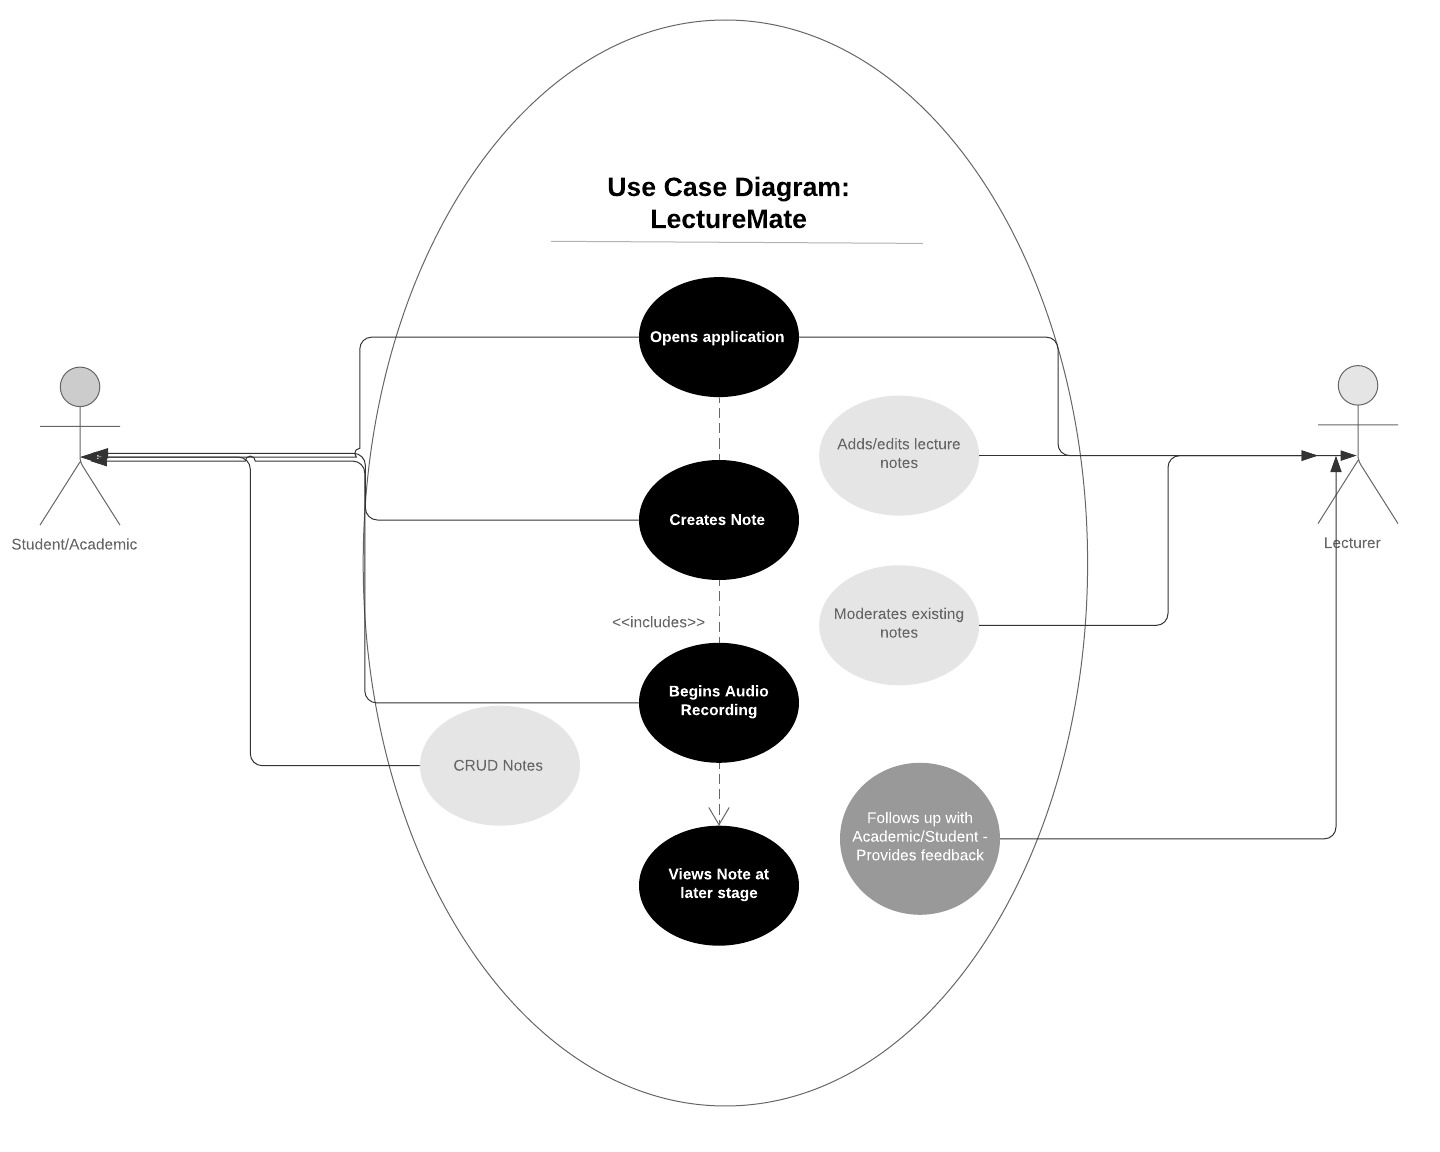
\includegraphics[width=\paperwidth]{/UseCase_UML.jpeg}}
			\end{center}
			\caption[Use Case Diagram]{Use Case Diagram}
		\end{figure}
	
\chapter{System Design}
	\section{Design Models}
		\subsection{Activity Diagram}
		\subsection{Sequence Diagram}
	\section{UI Design}

\chapter{Implementation}
	\section{Front End - Flutter}
	 Front end web development, also known as "client side programming", is based on everything that happens in the user's interface. From the layout, user interface and user experience, it is what the users can see and interact with. Since the project heavily focuses on the user base, it was essential that existing and potential clients feel comfortable with using the application. I established early on in the project that a mobile application would be best as it is the most easily accessible via multiple range of smart phones.\\
	
	The front end was handled by the Flutter package which makes use of the Material package as part of Flutter. This managed the UI and layout of the application. Due to the nature and simplicity of use of this package, it was very easy to look at making the UI aesthetically pleasing and pretty from the time of implementation - whereas I was expecting to have to focus more on the functionality of the application and then later look at making the UI more user friendly.

	\section{Business Layer - Flutter}
	The business layer which is the layer which handles the communication between the front-end and back-end operations - this is also written using Flutter as it has the ability to seamlessly link both the Flutter framework and the Google Firebase database. \\
	
	This consists of the database.dart file which acts as a database helper file containing the functions to submit and retrieve the data to and from the database. As well as this, due to potential unreliable internet connections, offline use has been considered where the audio recording is stored locally in case it has not been possible to upload to the database. \\
	
	Apart from this the other business layer functions are execute in smaller sections within classes in the code which can be seen in more depth in the Code Review section which proceeds after this.

	\section{Back End - Google Firebase}
	The back-end is managed entirely by Google Firebase, which as a Google product works well with Flutter which is also developed by Google. It is controlled through script written using the database helper which contains functions to execute CRUD functions in the database.\\

The database is a NoSQL database which is made up of collections, in the case of this application, a single collection 'notes' which contains documents which is each note uploaded in the application. The format of each note is the Tite, Body of the note, the Audio Recording URL and Recording Duration.\\

When being retrieved from the database, the application takes the URL of the audio recording and plays this back using the playback feature to add better functionality and ease of use to the users.

	\section{Mobile Application Development}
	Using Flutter has allowed the development of the application to be written once using the Flutter engine and can be used on both Android and iOS devices with no compatability issues which may depend on the platform.\\

This is a huge advantage as it allows the application to be deployed to users of both these devices and it can grow rapidly with continuous integration in potential developments in later revisions of the application. \\

The development and implementation phase was spread over a long period of four to five months whereby I was able to tackle each feature and spend a reasonable amount of time making sure that they would work as expected. Initally, I decided to focus on the functionality over the appearance and UI of the application. However, the ease of use of Flutter allowed the appearance to be worked on easily in a short space of time which working on the functionality. \\

I would utilise Version Control in the form of Git to manage the code and see the changes I had made to keep track of the progress made as well as have a backup in case of loss of work or to rollback changes which had caused major or significant issues to the application. This was very helpful as it  also meant I could review my code and spend time looking at whether any code was redundant or could be made redundant to simplify the code for clarity and speed when compiling the application at each stage.

	\section{Code Review}
	I reviewed the code I have for the application to explain the workings and how they contribute to the functionality. I will analyse and review each of the most important classes in the code to give a brief but clear understanding of their implementation:

		\subsection{database.dart}
		As previously mentioned, I have included a database helper file to manage the CRUD operation and functions between the front end application and Firebase database.\\

The way in which it works is firstly by using the packages to access the Firebase Storage (Firestore) and Database as well as packages used to store the timestamp of the notes (Intl) and to upload files (Dart.io).\\

Firstly, a new collection reference is crerated where the collection in the database, notes, is referred to and this is initalised so that all functions will access this to execute the operations:

			\subsubsection{uploadingNote}
			A condition is set to check whether a voice\_note has been added to the note, if not, the title, body and timestamp of the note are uploaded to the database. If an audio recording has been added, this is uploaded to Firebase Storage (Firestore) and the unique id is stored and is called in the upload of the note alongside the other parameters where the audio file URL will also be stored. 

			\subsubsection{getNotes}
			A List data structure is created to retrieve the list of notes in the database, referred to as a Snapshot. This reference is then used to get all the documents saved in the database, a for statement is then used to itemise each of the notes by the total there are stored and these are returned.

			\subsubsection{editNote}
			The notes collection is referenced and the document to be updated is retrieved using the document ID and this obtains the title and body of the note and in the editNote class this is displayed in the Text Editing Controllers to allow the user to make changes to the note.

			\subsubsection{deleteNote}
			This function simply deletes the note upon the users decision. Similar to the editNote function, it is referred to by its Document ID and then this is deleted.

		\subsection{newNote.dart}
		\begin{figure}[H]
			\begin{center}
	 		 	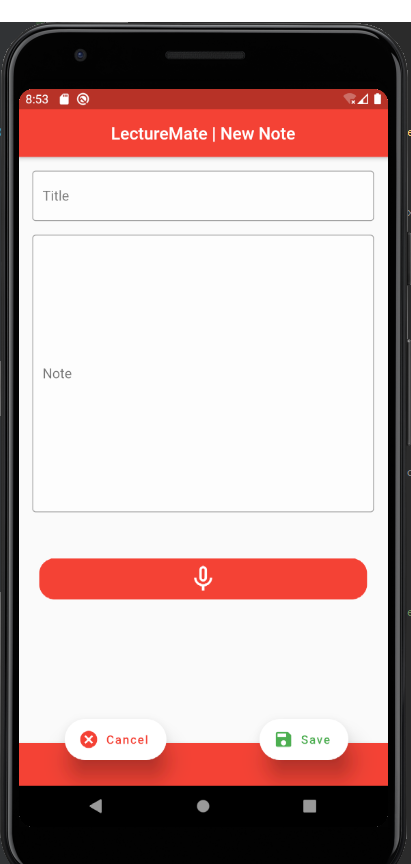
\includegraphics[width=3in]{/newnote.png}
			\end{center}
			\caption[New Note UI]{New Note UI}
		\end{figure}
		This class manages the operations used in creating a new note and the UI on the page.\\

Features of the New Note UI are the two text editing controllers containing the Title and Body of the note, as well as this, the Audio recording button which on press will begin recording and finally two buttons which cancel the note with a popup dialog for confirmation and a save button to save the data to the database.\\

This is very similar to the Edit Note UI, however, it does not display the audio recording feature as this only allows for updating and a recording cannot be updated as such, thus only the title and note body text controllers are modifiable.

		\subsection{list.dart}
		\begin{figure}[H]
			\begin{center}
	 		 	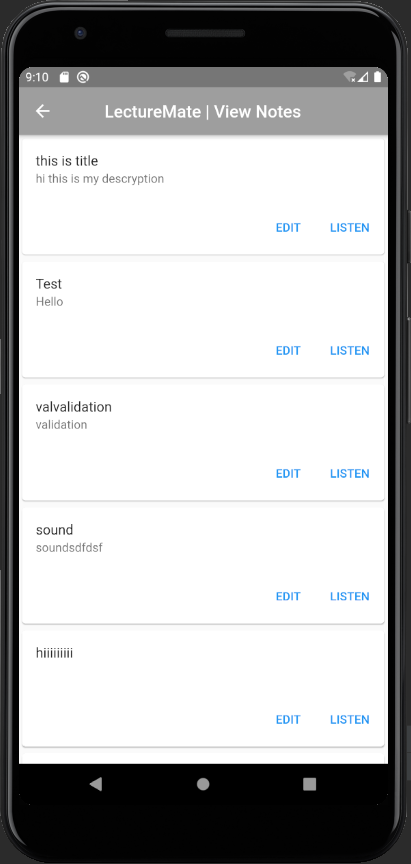
\includegraphics[width=3in]{/list.png}
			\end{center}
			\caption[View Notes UI]{View Notes UI}
		\end{figure}

		\subsection{playback.dart}
		\begin{figure}[H]
			\begin{center}
	 		 	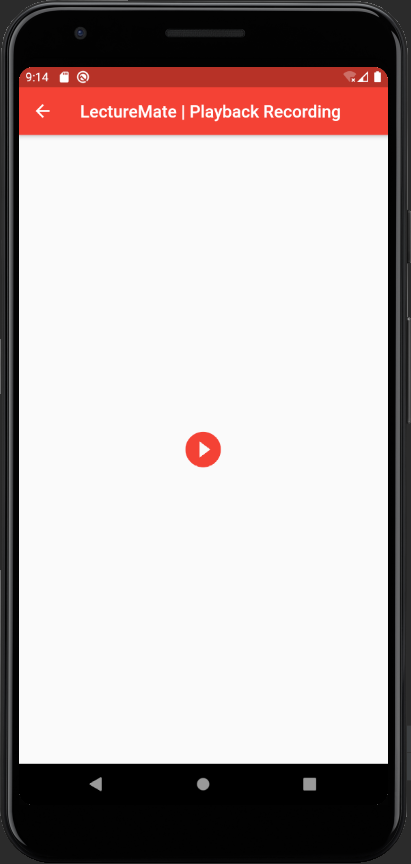
\includegraphics[width=3in]{/playback.png}
			\end{center}
			\caption[Recording Playback UI]{Recording Playback UI}
		\end{figure}

		\subsection{voice\_message.dart}
		\begin{figure}[H]
			\begin{center}
	 		 	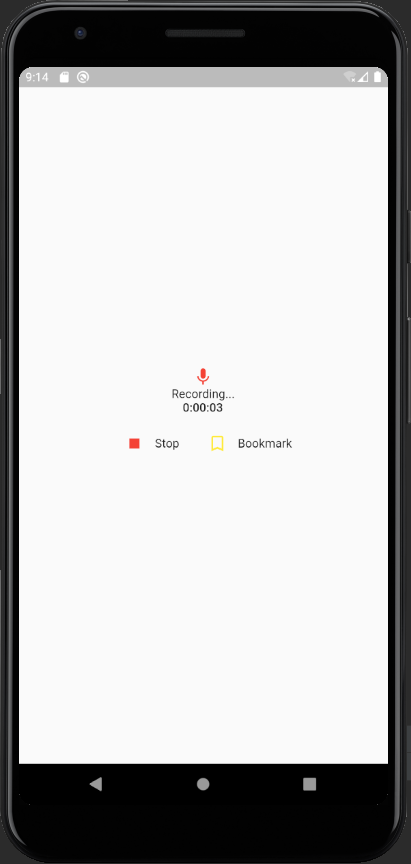
\includegraphics[width=3in]{/recording.png}
			\end{center}
			\caption[Record UI]{Record UI}
		\end{figure}

	\section{Disruptions and Solutions}
	\begin{center}
		\begin{figure}[H]
			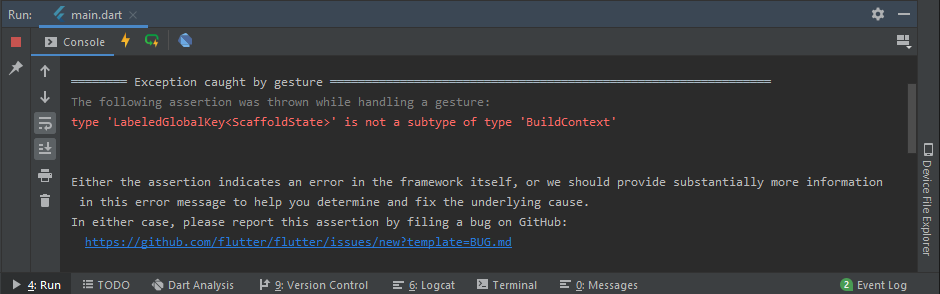
\includegraphics[width=6in]{/bug_1.png}
			\caption{Bug 1: Issue with Scaffold - Displaying the structure of the application}
		\end{figure}
		\begin{figure}[H]
			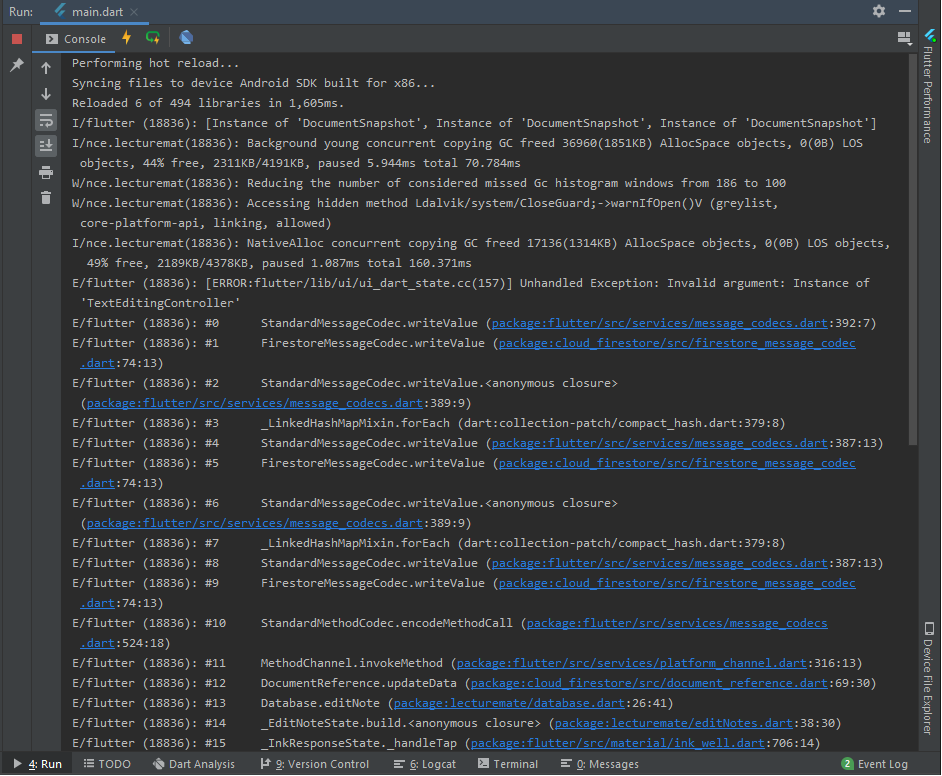
\includegraphics[width=6in]{/bug_2.png}
			\caption{Bug 2: Issue with retrieving data from Firebase}
		\end{figure}
	\end{center}

\chapter{Testing}
	\section{Testing Criteria}
	\section{Testing Results}
	\section{Formative Evalutation}
	\section{Functional Requirements Evaluation}
	\section{Non-functional Requirements Evaluation}

\chapter{Conclusion}
	\section{Summative Evaluation}
	\section{Potential Future Development}


\chapter{References}

\chapter{Appendix}

\newpage
\vspace*{\fill}
\begin{center}
\textbf{END OF DOCUMENT}
\end{center}
\vfill
\end{document}